\documentclass[UTF8]{ctexart}
\usepackage{mathtools,wallpaper}

\usepackage{t1enc}
\usepackage{pagecolor}
\usepackage{geometry}
\usepackage{diagbox}
\usepackage{graphicx}
\usepackage{wrapfig}
\usepackage{amssymb}

\geometry{left=2cm,right=2cm}

\begin{document}

\CTEXsetup[format={\Large\bfseries}]{section}
\title{实验报告}  
\author{徐亦昶 PB20000156}
\maketitle
\section{实验题目}声速的测量
\section{实验目的}
\begin{enumerate}
    \item 测量压电陶瓷换能器的谐振频率
    \item 用驻波法和相位比较法测量气体、液体中的声速
    \item 用时差法测量固体中的声速
\end{enumerate}
\section{实验原理}
声音在理想气体中的传播速度
\[v=\sqrt{\frac{\gamma RT}{M}}\]
在0摄氏度、1个大气压下,$v_0=331.45m/s$。
\newline
在摄氏温度$t^oC$时的声速
\[v_t=v_0\sqrt{1+\frac{t}{273.15}}\]
声速测量有如下几种方法:
\subsection{利用声速与频率、波长的关系测量}
设v为声速,$\lambda$为波长,f为频率,则它们有如下关系:
\[v=\lambda\cdot f\]
在实验中,声波的频率f等于数字频率计测得的电激励信号频率,或由低频信号发生器上的频率直接给出,而声波的波长$\lambda$则常用共振干涉法(驻波假设下)
和相位比较法(行波近似下)来测量。
\subsubsection{共振干涉法(驻波假设下)测声速}
\begin{figure}[h]
    \centering
    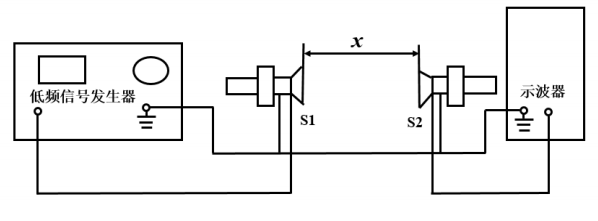
\includegraphics[scale=1]{共振干涉法.PNG}
    \caption{共振干涉法测量声速}
\end{figure}
如图,S1和S2分别为发射端和接受端,S2会将S1发送来的波反射,并使两个波干涉叠加。示波器中显示的是叠加波在S2处的声压。移动S2,示波器中显示的波幅会发生
周期性变化。不难发现S2实际上是在驻波上横向移动。一般地,当S1和S2的距离为半波长的整数倍时,声压的波幅最大,因此有关系式
\[n\frac{\lambda}{2}=|L_{n+1}-L_1|\]
连续改变距离L,并在每次声压波幅达到最大时测量相应的L,即可算出$\lambda$。
\subsubsection{相位比较法测量声速}
本方法是将S1发送的波和S2接受的波分别当作平面直角坐标系中的x和y,从而形成李萨如图形。假设开始李萨如图形是一条过一、三象限的直线,那么当S1和S2的
距离改变半个波长时,李萨如图形会变成过二、四象限的直线,再改变半个波长的距离,图形又会变为过一、三象限的直线。依次类推,多做几组实验,设第j组实验
中S1和S2的距离是$I_j$,拟合$I_j=\frac{\lambda}{2}j+b$即可求出$\lambda$。
\subsection{利用声波传播距离和传播时间计算声速}
本实验,要用到相距L的压电陶瓷换能器,其中一个利用逆压电效应把电能转换成发射出去的波,另一个利用正压电效应把接收到的波转换成电能。
利用$v=\frac{L}{t}$即可求出波速。
\section{实验内容}
\subsection{共振干涉法(驻波法)测声速}
\begin{enumerate}
    \item 将信号源的S1和双踪示波器的CH2分别连到测试仪接受和的发送端和接收端。
    \item 对示波器的分辨率、时间跨度等进行调整,知道上面显示出较为清晰的波。
    \item 在S1和S2的距离不变的条件下,调节信号源的频率(初始值设为34~38Hz比较好),使得示波器上显示的振幅最大。
    \item 在S1和S2相距5cm以上时,转动鼓轮移动S2,直到示波器上波幅达到最大,记录此时S1和S2的距离。注意不能反向转动鼓轮。
    \item 继续移动S2,当示波器上波幅最大时记录S1和S2的距离,依次连续记录12组数据。
    \item 利用最小二乘法求出半波长,并求出波速。
\end{enumerate}
\subsection{相位比较法测量水中的波长和声速}
\begin{figure}[h]
    \centering
    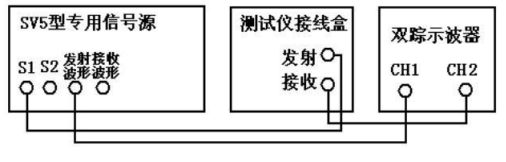
\includegraphics[scale=1]{相位法测量连线图.PNG}
    \caption{相位法测量连线图}
\end{figure}
\begin{enumerate}
    \item 如上图接线,并将示波器调至“X-Y”垂直振动合成模式,这时可观察到示波器上出现李萨如图形。
    \item 当S1和S2相距5cm以上时,转动鼓轮移动S2,使示波器上呈现直线。
    \item 移动鼓轮,依次测出李萨如图形斜率正、负变化的直线出现时S2的位置$L_i$,共记录8个位置值。
    \item 用作图法处理数据,求出半波长,进而得到波长和波速。
\end{enumerate}
\subsection{用时差法测量有机玻璃棒和黄铜棒中的声速}
\begin{figure}[h]
    \centering
    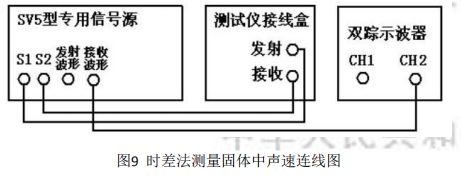
\includegraphics[scale=1]{时差法接线图.PNG}
    \caption{时差法测量固体中声速连线图}
\end{figure}
\newpage
\begin{enumerate}
    \item 如上图连线,并将测试仪接线盒调至“固体”模式。
    \item 选一根固体棒,使其两端连接到换能发射器上,并保证固体棒的两端面与两换能器的平面可靠、紧密接触。
    \item 把发射换能器尾部的连接插头插入接线盒的插座中。
    \item 记录信号源的时间读数,并测量固体棒的长度。
    \item 计算声波在该固体棒中传播的速度。
    \item 换另一根固体棒继续测量。
\end{enumerate}
\section{数据记录}
实验室室温:$25.0^oC$  
前两个实验中,f=37.04kHz
\begin{table*}[htbp]
    \centering
    \fontsize{8}{10}\selectfont
    \caption{共振干涉法(驻波假设下)测声速}
    \scalebox{1.15}{
    \begin{tabular}{|c|c|c|c|c|c|c|c|c|c|c|c|c|}
    \hline
    位置点& 1 & 2 & 3 & 4 & 5 & 6 & 7 & 8 & 9 &10&11&12 \\
    \hline
     S1、S2距离(cm)&15.53&15.08&14.60&14.13&13.65&13.17&12.70&12.24&11.77&11.32&10.85&10.36\\
     \hline
    \end{tabular}}
\end{table*}
\begin{table*}[htbp]
    \centering
    \fontsize{8}{10}\selectfont
    \caption{相位比较法测量声速}
    \scalebox{1.8}{
    \begin{tabular}{|c|c|c|c|c|c|c|c|c|}
    \hline
    位置点& 1 & 2 & 3 & 4 & 5 & 6 & 7 & 8\\
    \hline
     L(cm)&22.70&21.56&18.25&16.02&14.02&12.21&10.30&8.76\\
     \hline
    \end{tabular}}
\end{table*}
\begin{table*}[htbp]
    \centering
    \fontsize{8}{10}\selectfont
    \caption{时差法测量有机玻璃棒和黄铜棒中的声速}
    \scalebox{2}{
    \begin{tabular}{|c|c|c|}
    \hline
    \diagbox{材质}{物理量}&L(cm)&t($\mu s$)\\
    \hline
    黄铜棒&24.63&219\\
    \hline
    有机玻璃&17.98&116\\
    \hline
    \end{tabular}}
\end{table*}
\section{数据计算}
\subsection{共振干涉法(驻波假设下)测声速}
利用最小二乘法求得回归直线如图:
\begin{figure}[h]
    \centering
    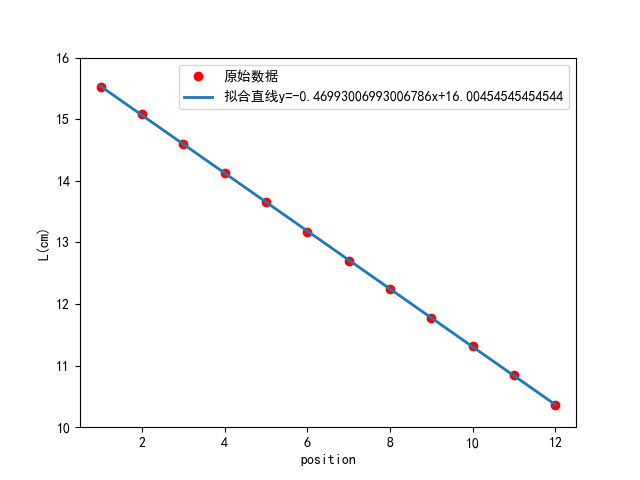
\includegraphics[scale=1]{共振干涉法数据.png}
    \caption{共振干涉法回归直线}
\end{figure}
\newpage
r=-0.99998  
\newline
先不考虑误差,可以求得$\lambda=0.94cm$,因此v=348.176m/s。
\newline
理论值$v_t=346.286m/s$。
\subsection{相位比较法测量声速}
仍然用作图法。
\begin{figure}[h]
    \centering
    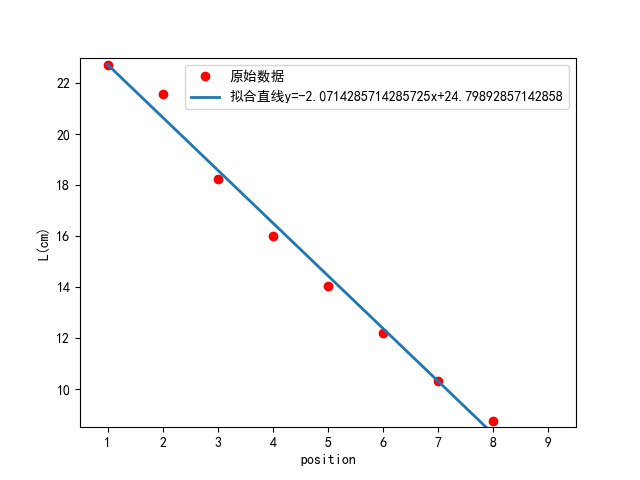
\includegraphics[scale=1]{相位法数据.png}
    \caption{LED的光强与电流关系(已扣除背景光强)}
\end{figure}
\newpage
r=-0.99542
\newline
可以求得$\lambda=4.14cm$,因此v=1533.456m/s。
\subsection{时差法测声速}
黄铜棒:$v=\frac{0.2463m}{219\mu s}=1124.66m/s$
\newline
玻璃棒:$v=\frac{0.1798m}{116\mu s}=1550.00m/s$
\newpage
\section{不确定度分析}
仅对第一个实验分析。
\newline
使用origin可以得到斜率的标准差为$9.532\times 10^{-4}$,因此波长的
标准差$S_{\lambda}=1.9064\times 10^{-3}cm$。所以$\lambda$的A类不确定度
$u_A=\frac{S_{\lambda}}{\sqrt{n}}=5.503\times 10^{-4}cm$。当置信概率P=0.95时,t因子
$t_{0.95}=2.26$。游标卡尺最大允差0.05mm,估计误差可忽略不计(比仪器误差小得多)。
因此$\Delta_B=5\times 10^{-3}cm$。由于所用仪器符合正态分布,所以C=3,且$t_P=1.96$,所以
B类不确定度$u_B=\frac{\Delta_B}{C}=1.67\times 10^{-3}$。
\newline
所以合成不确定度$U_{0.95}=\sqrt{\left( t_{0.95}\cdot u_A \right)^2+\left( t_P\cdot u_B \right)^2}=0.01cm$
因此v的不确定度为$0.01\times 37040\div 100=3.704m/s$。
\newline
因此$v=\left( 348.176\pm 3.704 \right)m/s$,理论值恰好落在这个范围内。
\section{思考}
\begin{enumerate}
    \item 声音在传播的过程中会不断衰减,所以随着距离的增加,声压振幅极大值会减小。
    \item 不同点在于驻波法、相位法通过测量波长来确定波速,而时差法通过速度公式直接计算波速,
    且前两种方法测量波长的方式不同,一个是通过驻波,另一个是直接通过相位变化。相同点在于它们都是通过
    声波的物理性质来间接测量波速,且前两种方法都是通过波长和频计算波速。
    \item 不相同,因为不同介质杨氏模量不同。
\end{enumerate}

\end{document}